\documentclass{article}
\usepackage[utf8]{inputenc}
\usepackage{graphicx}
\usepackage{amsmath,amsthm,amsfonts,amssymb,dsfont,mathtools}
\usepackage[portuguese]{babel}
\usepackage{csquotes}
\usepackage{url}


\title{Cálculo Diferencial e Integral I}
\author{Lívia Lima Bion }
\date{16 de Setembro de 2022}

\begin{document}

\maketitle

\section{Introdução}
\paragraph{}
A origem do estudo do Cálculo foi na Grécia Antiga, onde a busca por soluções sobre problemas geométricos levou ao aprimoramento dessa ciência, e com o passar dos anos, ao se concretizar, mostra-se presente no conteúdo da disciplina “Cálculo Diferencial Integral I”. Um dos problemas enfrentados na Antiguidade foi: O Método da Exaustão. Esse método foi criado a fim de resolver um problema conhecido como o Problema da Área, que ainda é bastante debatido e posto nas salas de aula da disciplina de Cálculo I. \cite{Matematica}

Além da parte histórica, essa disciplina traz outros tipos de debates que são mais recentes, como o problema da reta tangente. Atualmente, o estudo de Cálculo Diferencial e Integral se expande para várias áreas de conhecimento e sua origem foi buscar soluções para problemas comuns, mas complexos o suficiente para ser desenvolvida tal técnica de raciocínio. 

Ainda nesse artigo, serão contempladas mais informações sobre essa disciplina, como: sua estrutura de conteúdos; sua relevância para a computação; e sua relação com outras disciplinas.

\section{Estrutura de conteúdos}
\paragraph{}
Na Universidade Federal de Pernambuco, a disciplina é dividida em três unidades, onde ao longo delas se constrói um raciocínio construtivo acerca dos conteúdos:\cite{disciplina}

\subsection{Primeira Unidade:}
\begin{itemize}
\item Limites
\item Derivadas
\item Regras de derivação
\end{itemize}

\subsection{Segunda Unidade:}
\begin{itemize}
\item Regra de L’ Hôspital
\item Teorema do valor médio
\item Esboço de gráficos
\end{itemize}

\subsection{Terceira Unidade:}
\begin{itemize}
\item Áreas e distâncias
\item Teorema Fundamental do Cálculo
\item Integrais e regras de integração
\end{itemize}

\section{Relação com outras diciplinas}
\paragraph{}
No perfil curricular de Ciência da Computação na UFPE a disciplina de Cálculo I não tem pré-requisito, justamente por estar no primeiro período da graduação. Além disso, não é necessário pagar nenhuma cadeira ao mesmo tempo que ela (co-requisito).

Dando continuidade, a disciplina de Cálculo Diferencial e Integral I é pré-requisito de mais três disciplinas obrigatórias: Estatística e Probabilidade para computação (ET586), Física para Computação (FI582) e Processamento Gráfico (IF680). E ainda pode-se encontrar pré-requisito de Cálculo I em algumas eletivas como: Cálculo Avançado para Computação (IF764) e Processamento de Sinais (IF753).\cite{perfil}

\section{Relevância}
\paragraph{}
Ainda que possa parecer que a disciplina de Cálculo Diferencial e Integral I não seja importante para a formação das pessoas em Ciência da Computação, na verdade é muito importante sim. O pensamento matemático, não só abordado no Cálculo mas também em diversas outras cadeiras, auxilia no desenvolvimento do pensamento lógico que se precisa ter e aprimorar para desenvolver um projeto de programação. Essa disciplina não foge desse molde, inúmeros conceitos abordados durante a matéria são aproveitados na área da computação, como entender e analisar o comportamento de funções. Isso, em conjunto com o assunto do tópico anterior (pré-requisitos), forma a relevância dessa disciplina para a formação do Cientista da Computação.\cite{importancia}

\section{Problema da Tangente}
\paragraph{}

A disciplina de Cálculo I, traz esse conceito ao longo do período, que é um raciocínio importante para dar continuidade ao estudo de Cálculo.

O Problema da Reta Tangente é um dos primeiros raciocínios abordados na disciplina, pois ele é responsável por criar a noção intuitiva do que é o limite.\cite{JamesS}

É traçada uma reta “t” (roxa) tangente a uma curva no ponto P, também existirá uma reta secante azul que irá tocar a curva nos pontos P e Q.

\begin{figure}[ht]
    \centering
    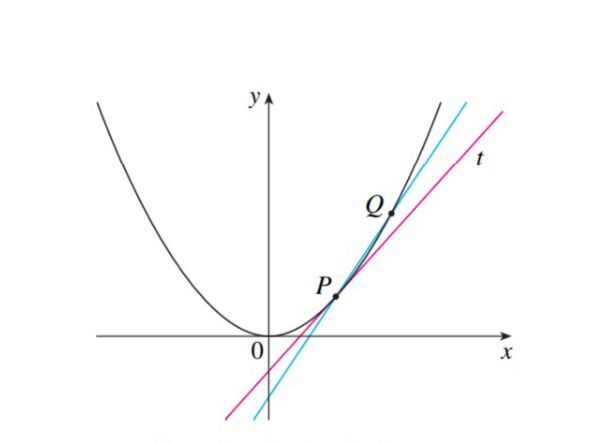
\includegraphics[width=7cm]{imagens/tangente_1.jpg}
    \caption{A figura mostra duas retas, uma secante (azul) a curva e uma tangente(roxa) a curva. E os pontos: P que pertencem a ambas das retas e o Q que só pertence a reta secante. \cite{JamesS}}
    \label{figura:tangente1}
\end{figure}

\paragraph{}
Pode-se observar que entre a figura 1 e 2, o ponto Q está tendendo ao ponto P. Ou seja, estão se aproximando. E isso está acontecendo para que a inclinação da reta t seja igual ao da reta azul

\begin{figure}[ht]
    \centering
    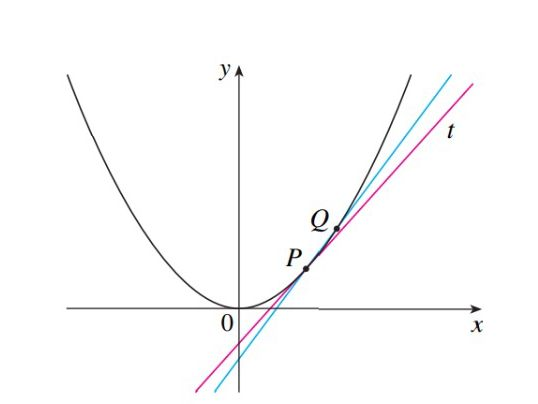
\includegraphics[width=7cm]{imagens/tangente_2.jpg}
    \caption{Os pontos P e Q na curva vão se aproximando a partir da mudança da inclinação da reta azul \cite{JamesS}}
    \label{figura:tangente2}
\end{figure}

\paragraph{}
Se chamarmos a inclinação da reta roxa de “mr” e a da reta azul de “ma”, podemos observar que: \[mr = \lim_{Q \to P} ma\]
E essa expressão representa a sobreposição dos dois pontos.


\section{Conclusão}
\paragraph{}
Logo, foi visto desde como surgiu o estudo da disciplina até as nuances dela na Universidade Federal de Pernambuco. Portanto, a visão de dentro e de fora do meio acadêmico mostra o raciocínio que a disciplina proporciona e a importância dela para a carreira de um cientista da programação.

\bibliographystyle{abbrvnat}
\bibliography{ref}
\end{document}
